\section{ZONES OF CONTROL}

\begin{wrapfigure}{R}[-5pt]{2cm}
  \raggedleft
  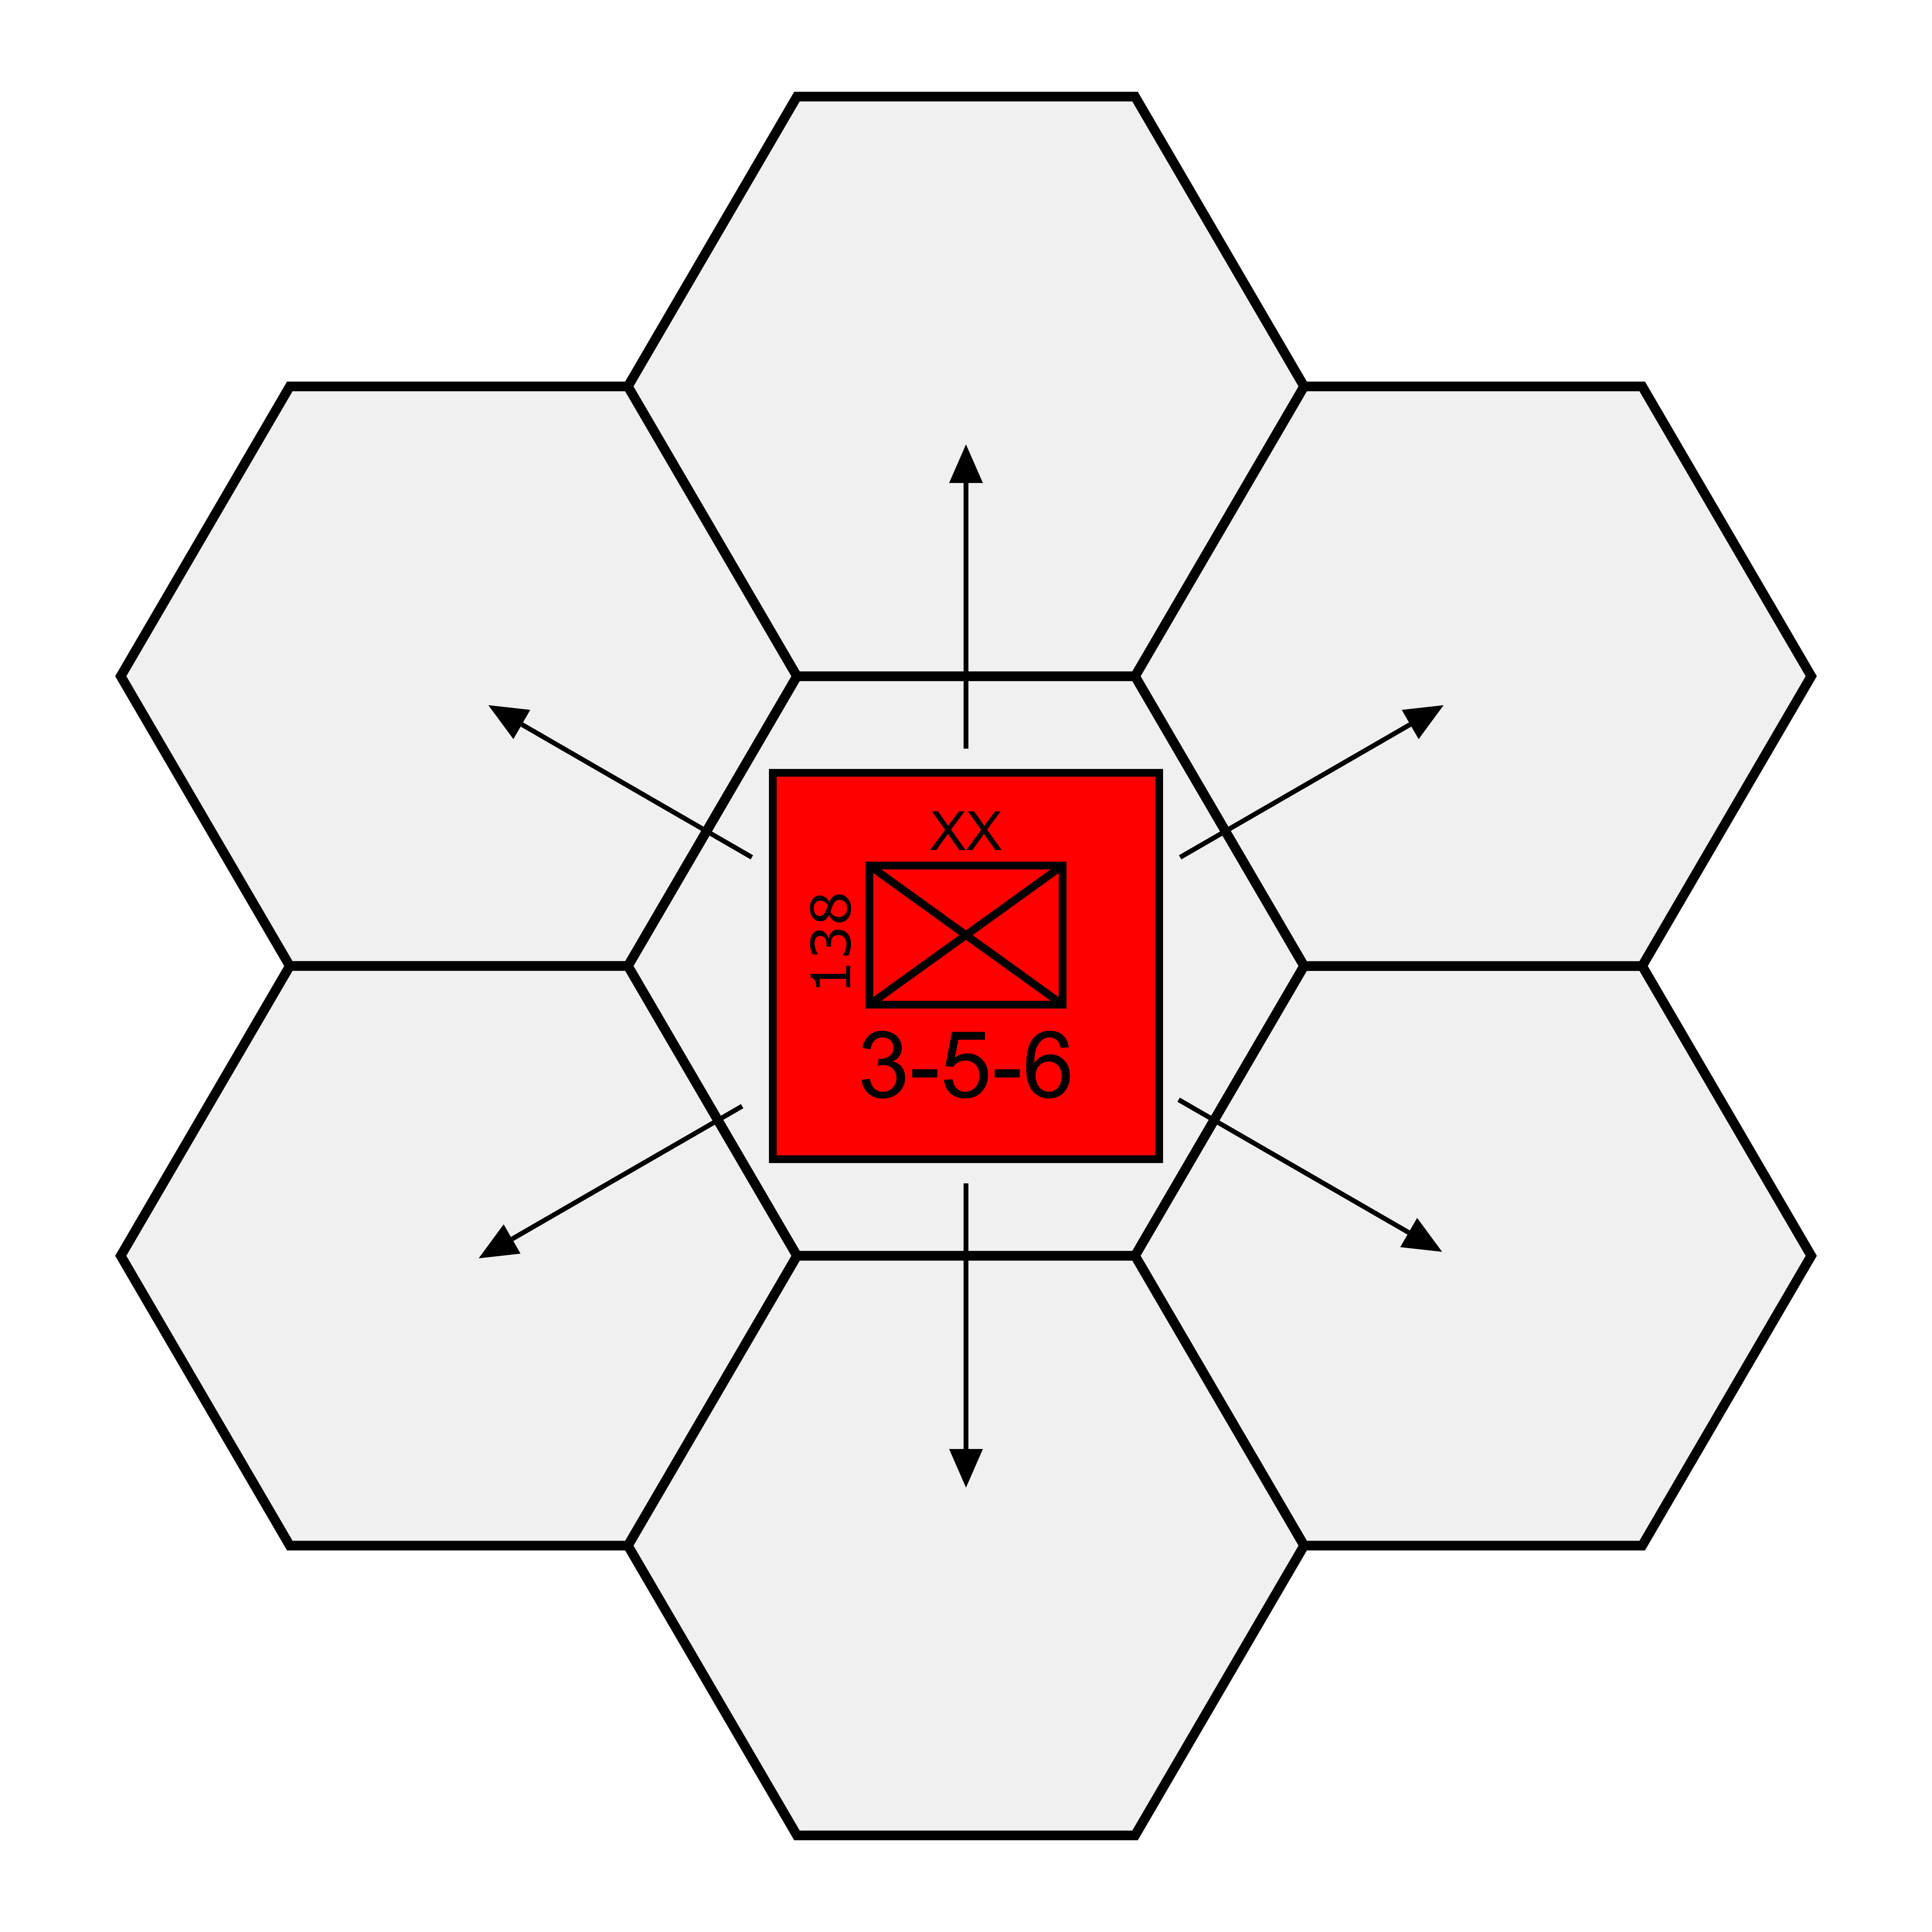
\includegraphics[width=0.1\textwidth]{zoc_display.png}
\end{wrapfigure}

GENERAL RULE:

The six hexagons surrounding a hex constitute the Zone of Control (ZOC) of any units in that hex. Hexes upon which a unit exerts a Zone of Control are called controlled hexes, and inhibit the movement of Enemy units. All units must cease movement when they enter an Enemy-controlled hex and may not leave that hex voluntarily.

CASES:

\subsection{EFFECTIVENESS OF\\*ZONES OF CONTROL}

\subsubsection{} All units exert a Zone of Control at all times during the entire Game-Turn,unless they are in a state of Disruption. Disrupted units have no ZOC.

\subsubsection{} Units never pay any additional cost to enter an Enemy-controlled hex.

\subsubsection{} Units may never voluntarily leave an Enemy controlled hex. Friendly units may leave Enemy-controlled hexes only as a result of combat. However, see Overrun Rules in Case 6.5.

\subsubsection{} Friendly units (but \textbf{not} Friendly ZOC's) negate the presence of Enemy Zones of Control for the purposes of tracing Supply Lines and Leadership Radii. They do not negate Enemy Zones of Control for purposes of movement. They also negate the effect of an Enemy ZOC for the purposes of retreat.

\subsubsection{} If a given unit is in an Enemy-controlled hex, the Enemy unit is also in its Zone of Control. The two units are equally and jointly affected.

\subsubsection{} Zones of Control extend into all six hexes adjacent to the controlling unit's hex. Zones of Control extend across River hexsides; however, they do \textbf{not} extend across all-Lake hexsides. No other terrain affects Zones of Control.

There is no additional effect of having more than one unit exerting its Zone of Control onto a given hex.